\documentclass[a4paper,11pt]{jarticle}

% レイアウト
\setlength{\hoffset}{0cm}
\setlength{\oddsidemargin}{-3mm}
\setlength{\evensidemargin}{-3cm}
\setlength{\marginparsep}{0cm}
\setlength{\marginparwidth}{0cm}
\setlength{\textheight}{24.7cm}
\setlength{\textwidth}{17cm}
\setlength{\topmargin}{-45pt}


\renewcommand{\baselinestretch}{1.2}
\renewcommand{\floatpagefraction}{1}
\renewcommand{\topfraction}{1}
\renewcommand{\bottomfraction}{1}
\renewcommand{\textfraction}{0}
\renewcommand\thefootnote{\arabic{footnote})}

% パッケージ
\usepackage[dvipdfmx]{graphicx}
\usepackage{amsmath,amssymb,epsfig}
\usepackage{eucal}
\usepackage{bm}
\usepackage{ascmac}
\usepackage{pifont}
\usepackage{multirow}
\usepackage{enumerate}
\usepackage{cases}
\usepackage{type1cm}
\usepackage{cancel}
\usepackage{url}
\usepackage{cite}
%\usepackage{color}
\usepackage[dvipdfmx]{color}
\usepackage{caption}
\usepackage[caption=false]{subfig}
\captionsetup[figure]{labelsep=space}
\usepackage{here}
\usepackage{listings}

% 擬似コード作成用
\usepackage[ruled,vlined]{algorithm2e}
\usepackage{setspace}
\input{../sty/jdummy.def}

% カウンタの設定
\setcounter{section}{0}
\setcounter{subsection}{0}
\setcounter{subsubsection}{0}
\setcounter{equation}{0}

% キャプションの図をFigに変更
\renewcommand{\figurename}{Fig.}
\renewcommand{\tablename}{Tab.}

% 式番号を式(章番号.番号)に
\makeatletter
\renewcommand{\theequation}{\arabic{equation}}
\@addtoreset{equation}{section}
\makeatother

% ソースコードの設定
%\lstnewenvironment{mylisting}[1][]

%frame=single, number=left, tabsize=2}

% タイトル部分
\title{\vspace{-20truemm}
{\normalsize \rightline{平成29年\ 11月\ 8日}}
{\large 確率システム制御特論\\}
第8回演習問題\\
\date{}
\vspace{-2truemm}}
\author{機械知能工学専攻 知能制御工学コース \hspace{3mm} 17344219 \ 二宮 悠二}
%---------------------------------------------
% ドキュメントの開始
\begin{document}
% ソースコードの設定
\definecolor{OliveGreen}{cmyk}{0.64,0,0.95,0.40}
\definecolor{colFunc}{rgb}{1,0.07,0.54}
\definecolor{CadetBlue}{cmyk}{0.62,0.57,0.23,0}
\definecolor{Brown}{cmyk}{0,0.81,1,0.60}
\definecolor{colID}{rgb}{0.63,0.44,0}

\lstset{
  language=Pascal,
  basicstyle={\ttfamily\small},
  keywordstyle={\color{OliveGreen}},
  keywordstyle={[2]\color{colFunc}},
  keywordstyle={[3]\color{CadetBlue}},
  commentstyle={\color{Brown}},
  identifierstyle={\color{colID}},
  stringstyle=\color{blue},
  tabsize=2,
  frame=trBL,
  numbers=left,
  numberstyle={\ttfamily\small},
  breaklines=true,
  backgroundcolor={\color[gray]{.95}},
  %captionpos=\textbf{}
}
%---------------------------------------------
\parindent = 0pt % 字下げoff
% 表紙
\titlepage
\maketitle
%---------------------------------------------
% 課題内容
{\Large{\bf 問題}}
%---------------------------------------------
\vspace{2mm}\\
\ \ 第7回の課題で構築したシミュレーション環境を利用して,テキストp.161〜以降の拡張カルマンフィルタを構築せよ.ソースコードとシミュレーション結果を提出すること.\\\\
%---------------------------------------------
{\Large{\bf 解答}}
%---------------------------------------------
\vspace{2mm}\\
\ \ 本課題では,次のスカラの非線形状態方程式
%-----------------------------------
\begin{eqnarray}
 && x(k+1) = x(k) + 3{\rm cos}\dfrac{x(k)}{10} + v(k), ~~ x(0) = 10 \\
 && y(k) = x^3(k) + w(k)
\end{eqnarray}
%-----------------------------------
で記述される非線形時系列$ y(k) $をフィルタリングする問題を考えた.その結果を{\bf Fig.}\ref{fig:sim}に,その時のソースコードをListing 1に示す.なお,本課題ではPythonを用いてプログラムの作成を行ない,$ k = 50 $までのデータに対しシミュレーションを実行した.
\newpage
%-----------------------------------
\begin{figure}[tb]
 \begin{center}
  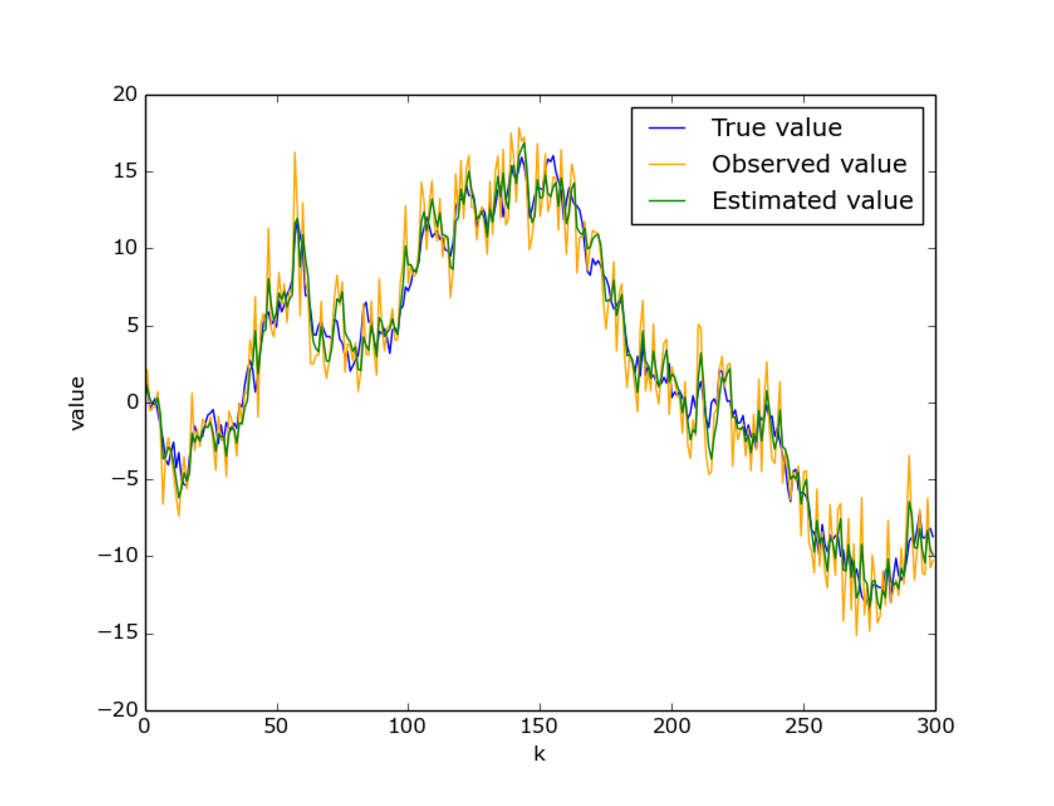
\includegraphics[scale=0.9]{../figure/eps/sim.eps}
  \caption{例題6.1のシミュレーション結果}
  \label{fig:sim}
 \end{center}
\end{figure}
%-----------------------------------
\begin{lstlisting}[basicstyle=\ttfamily\footnotesize,frame=single,numbers=left,language=Python,caption=ソースコード]
#!/usr/bin/env python
# -*- coding: utf-8 -*-
# python3.5

import numpy as np
import matplotlib.pyplot as plt

def lkf(y,sigmav2,sigmaw2,A,b,c,p): # Define the Kalman Filter

    x_hat = []
    x_hat_pri = 0.0

    for y_k in y:
        x_pri = A * x_hat_pri
        p_pri = A * p + sigmav2 * b * b
        g = (p_pri * c) / (c * p_pri * c + sigmaw2)
        x_hat_next = x_pri + g * (y_k - c * x_pri)
        p = (1 - g * c) * p_pri
        x_hat_pri = x_hat_next
        x_hat.append(x_hat_next)
        np.array([x_hat])

    return x_hat

def main():

    # Set parameter
    A = 1.0
    b = 1.0
    c = 1.0

    p = 0.0

    sigmav2 = 1.0
    sigmaw2 = 2.0

    # Number of sample
    n = 300
    N = np.linspace(0, n-1, n)

    # Make noise
    v = np.random.normal(0,sigmav2,n)
    w = np.random.normal(0,sigmaw2,n)

    # Create dataset
    x = []
    sum_v = 0
    for v_k in v:
        sum_v += v_k
        x.append(sum_v)
        np.array([x])

    y = x + w

    # Kalman Filter
    x_chil = lkf(y,sigmav2,sigmaw2,A,b,c,p)

    # Plot
    plt.figure(figsize=(8, 6))
    plt.plot(N,x,label="True value",color="blue",linewidth=1)
    plt.plot(N,y,label="Observed value",color="orange",linewidth=1)
    plt.plot(N,x_chil,label="Estimated value",color="green",linewidth=1)
    plt.xlabel("k")
    plt.ylabel("value")
    plt.legend()
    plt.show()

if __name__ == '__main__':
    main()
\end{lstlisting}
%-----------------------------------


% % 表の挿入

% \begin{table}[htb]
%   \begin{center}
%     \caption{各素子のパラメータ}
%     \begin{tabular}{c|c|c} \hline
%       定数名[単位] & 記号 & 値 \\ \hline \hline
%       周波数[Hz] & $f_U,f_V,f_W$ & 120 \\ \hline
%                      & $\phi_U$ & $\frac{2\pi}{3}$ \\
%       初期位相角[rad] & $\phi_V$ & $\frac{4\pi}{3}$ \\
%                      & $\phi_W$ & $2\pi$ \\ \hline
%       抵抗[$\Omega$] & $R$ & 10 \\ \hline
%     \end{tabular}
%     \label{param}
%   \end{center}
% \end{table}


% % 図の挿入

% \begin{figure}[tb]
%  \centering
%  \vspace{0.5cm}
%  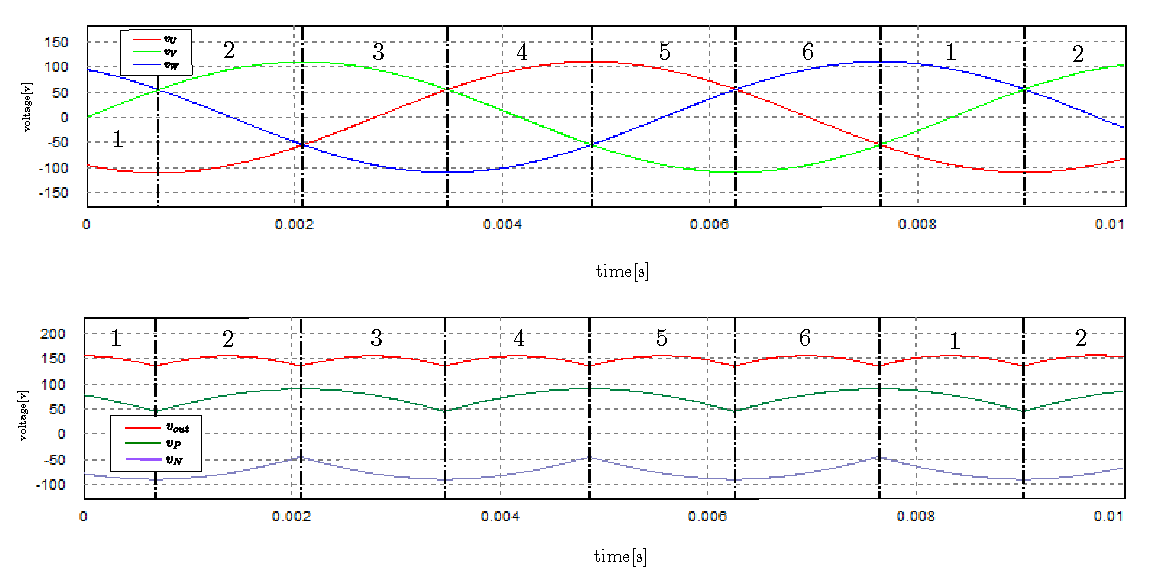
\includegraphics[scale=0.85]{../figure/waves.eps}\\
%  \hspace{0.0cm}
%  % 入力と出力\\
%  % \\
%  % \vspace{1.2cm}
%  % 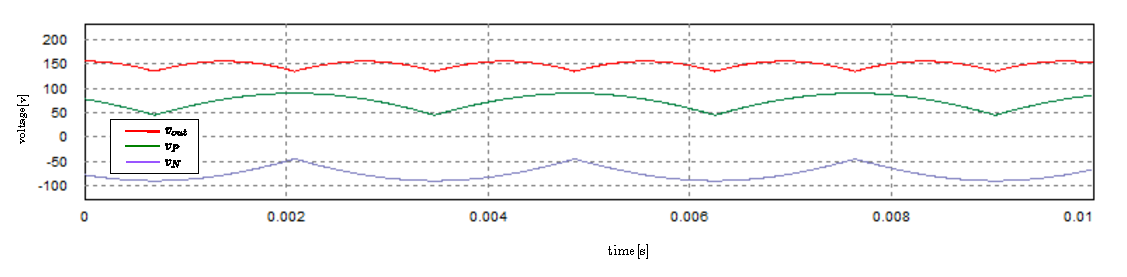
\includegraphics[scale=0.825]{../figure/output.eps}\\
%  % (b) 出力の電位\\
%  % \\
%  \caption{シミュレーションにより得られた各電源電圧(上)と出力電位(下)の波形}
%  \label{wave}
% \end{figure}

% \newpage

% % 図を並べて挿入

% \begin{figure}[tb]
%  \centering
%  \subfloat[区間1における回路動作]{\includegraphics[scale=0.5]{../figure/kukan_1.eps}}
%  \hspace{1.5cm}
%  \subfloat[区間2における回路動作]{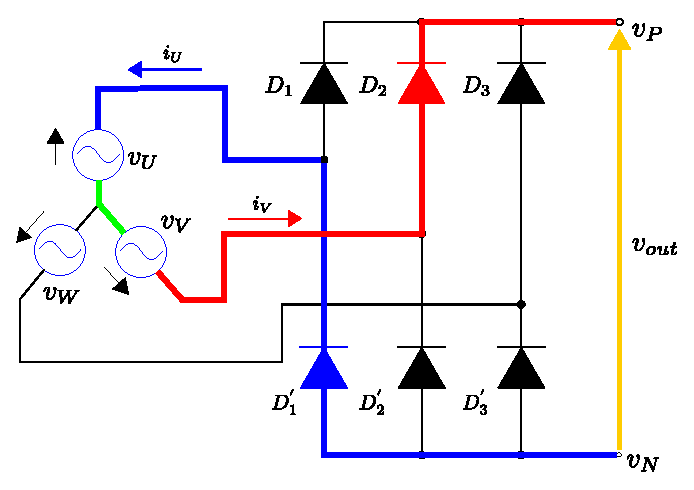
\includegraphics[scale=0.5]{../figure/kukan_2.eps}}
% \\
%  \vspace{0.5cm}
%  \subfloat[区間3における回路動作]{\includegraphics[scale=0.5]{../figure/kukan_3.eps}}
%  \hspace{1.5cm}
%  \subfloat[区間4における回路動作]{\includegraphics[scale=0.5]{../figure/kukan_4.eps}}
% \\
%  \vspace{0.5cm}
%  \subfloat[区間5における回路動作]{\includegraphics[scale=0.5]{../figure/kukan_5.eps}}
%  \hspace{1.5cm}
%  \subfloat[区間6における回路動作]{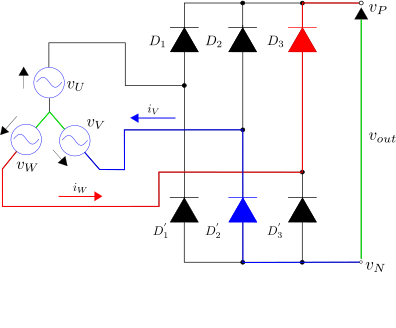
\includegraphics[scale=0.5]{../figure/kukan_6.eps}}
% \\
%  \caption{各区間での回路動作の様子}
%  \label{circuit_kaku}
% \end{figure}

% % 文中へのラベリング
% {\bf Fig. }\ref{circuit_kaku}に示す〜

% 参考文献
\begin{thebibliography}{99}
\addcontentsline{toc}{section}{参考文献}
\bibitem{1} 足立 修一・丸田 一郎,”カルマンフィルタの基礎”,東京電機大学出版局,pp.112-117,2012.
%\bibitem{data} UCI Machine Learning Repositiry,SECOM Data Set,https://archive.ics.uci.edu/ml/datasets/SECOM,(最終閲覧日:2017年10月18日).
\end{thebibliography}

\end{document}
